\documentclass[conference]{IEEEtran}
\IEEEoverridecommandlockouts
% The preceding line is only needed to identify funding in the first footnote. If that is unneeded, please comment it out.
\usepackage{cite}
\usepackage{amsmath,amssymb,amsfonts}
\usepackage{systeme}
\usepackage{algorithmic}
\usepackage{graphicx}
\usepackage{textcomp}
\usepackage{xcolor}
\usepackage{flushend}
\usepackage{float}
\usepackage{lmodern}
\usepackage[]{algorithm2e}
\usepackage{times}
\usepackage[bookmarks=false]{hyperref}
\usepackage{pgfplots}
\usepackage{booktabs}
\usepackage{subfigure}
\usepackage[a4paper, left=0.51in, right=0.51in, top=0.75in, bottom=1.69in]{geometry}
\usepackage{listings}
\lstset{
	% --- Estilo da Fonte ---
	basicstyle=\ttfamily\small,   % Fonte: monoespaçada e pequena.
	% --- Estilos de Sintaxe (COM CORES) ---
	keywordstyle=\color{blue}\bfseries, % Palavras-chave: azul e negrito.
	commentstyle=\color[rgb]{0.1,0.5,0.1}, % Comentários: verde escuro.
	stringstyle=\color{red},            % Strings ("texto"): vermelho.
	% --- Formatação ---
	showstringspaces=false,       % Não marca espaços em strings.
	breaklines=true,              % Quebra linhas longas.
	frame=single,                 % Borda simples (caixa).
	numbers=left,                 % Números à esquerda.
	% --- Estilo dos Números (NOVO) ---
	numberstyle=\tiny, % Tamanho reduzido e cor cinza
	xleftmargin=20pt,       % Empurra todo o bloco de código para a direita, afastando-o da coluna vizinha
	framexleftmargin=15pt,
}

\newcommand{\sandro}[1]{{\color{red}[#1]}}		
\newcommand{\lucas}[1]{{\color{blue}[#1]}}


\def\BibTeX{{\rm B\kern-.05em{\sc i\kern-.025em b}\kern-.08em
    T\kern-.1667em\lower.7ex\hbox{E}\kern-.125emX}}
    
    \IEEEoverridecommandlockouts
\IEEEpubid{%
\makebox[\columnwidth]{%
978-1-7281-7539-3/20/\$31.00~\copyright{}2020 IEEE\hfill%
} \hspace{\columnsep}\makebox[\columnwidth]{ }%
}
\begin{document}

\title{\noindent 
		\begin{minipage}[c]{0.1\textwidth}
			
\includegraphics[width=2.2cm]{Imagens/logo} 
		\end{minipage}
		\begin{minipage}[c]{0.8\textwidth}
			\centering 
			\fontsize{12}{14}\selectfont
			Universidade Federal de Itajubá - UNIFEI - Campus Itabira \\
			Curso de Engenharia da Computação - ECO \\
			Computação Gráfica e Processamento Digital de Imagens  \\
			Prof. Dr. André Ribeiro de Brito
		\end{minipage}
	}

\author{\IEEEauthorblockN{Fabrício Rickelmer Souza Duarte }
	\IEEEauthorblockA{Instituto de Ciências Tecnológicas, Universidade Federal de Itajubá, Itabira, Minas Gerais, Brazil}
	\textit{d2023012884@unifei.edu.br} \\
	\text{R.A: 2023012884}}
	
\maketitle

\begin{abstract}
	Esse artigo tem como fundamento a implementação de um algoritmo genético utilizando mutações, cruzamentos e torneios para a procura de horários ideais e preços baseado em um arquivo de texto para o estudo da matéria de Inteligencia Artificial ministrada na UNIFEI pelo professor Sandro Carvalho Izidoro.
\end{abstract}
\renewcommand\IEEEkeywordsname{Keywords}
\begin{IEEEkeywords}
	Genético, algoritmo, viagens, torneio, cruzamento, mutação, população.
\end{IEEEkeywords}

%----------------------------------------------------

\section{Introdução}

\subsection{Problema Escolhido}

Foi escolhido a atividade 1 do trabalho passado, que era sobre implementar um Algoritmo Genético para
otimizar os valores das passagens e os horários dos voos, procurando o menor tempo de espera e custo monetário.

\begin{figure}[htb]
	\centering
	
	\caption{Pesquisadores e suas respectivas cidades com destino a Roma.}
	\vspace{0.2cm}
	
	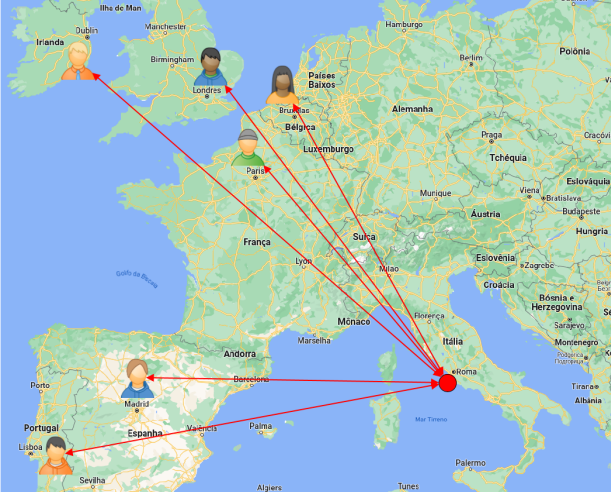
\includegraphics[width=\linewidth]{Imagens/Mapa}
	
	{\footnotesize Fonte: Autor Sandro Izidoro (2026).}
\end{figure}

Os dados que serviram de espaço de busca foram retirados do "flights.txt", que possuía lugares de saída e chegada, hora de saída e chegada; Passados junto ao documento do trabalho.

\subsection{Funcionamento do GA}

É um algoritmo bio inspirado que visa encontrar os melhores tipo de solução de um problema dado baseado em variáveis determinadas. Ele não leva em conta todas as possibilidades do cenário biológico inspirado, existe um certo grau de abstração para ele poder ser levado a um código computacional.

\subsubsection{Variáveis}

Esse são os parâmetros principais do GA, que vão garantir o seu funcionamento de forma eficaz.

\begin{itemize}
	\item int tam\_Populacao = 15; \\
	O espaço de busca não era tão grande então não foi utilizado um tamanho de população alto.
	\item int geracoes = 100; \\
	Número maior pra procurar todas as possibilidades possíveis.
	\item float prob\_Cruzamento = 0.80; \\
	O cruzamento alto garante herança de bons padrões para o algorítimo.
	\item float prob\_Mutacao = 0.05; \\
	Baixo pra não ocorrer a geração bem próxima da aleatoriedade.
	\item int tam\_torneio = 2; \\
	Nesse tipo de situação o tamanho 2 é o mais certo pra garantir que genes dominantes não tomem conta do algoritmo.
\end{itemize}

%----------------------------------------------------

\section{Desenvolvimento}

\subsection{Bibliotecas Utilizadas}

\subsubsection{C++}

\begin{itemize}
	\item $<$iostream$>$ \\
	Responsável pela entrada e saída padrão do sistema. Utilizada no código para exibir os relatórios de progresso, o resumo do melhor indivíduo encontrado, além de mensagens de sucesso e alertas de erro diretamente no terminal de execução.
	
	\item $<$fstream$>$ \\
	Biblioteca responsável pela manipulação de arquivos do disco rígido. Foi utilizada através do comando ifstream para abrir e ler o banco de dados inicial (flights.txt), e do comando ofstream para criar, nomear e gravar os dados exportados (como os relatórios de texto .txt e a planilha de dados estatísticos .csv).
	
	\item $<$sstream$>$ \\
	Ferramenta de conversão e processamento estruturado de strings. Na função de verificação e leitura do arquivo de voos, transforma cada linha de texto em um fluxo contínuo de dados (String Stream), permitindo isolar as informações delimitadas por vírgulas (origem, destino, horários e preço) para conversão numérica.
	
	\item $<$vector$>$ \\
	Fornece a estrutura de dados de listas dinâmicas, que expandem de tamanho automaticamente na memória. Atua como a espinha dorsal de armazenamento do programa, sendo utilizada para guardar o espaço de busca inicial, agrupar os voos selecionados para compor o cromossomo, gerenciar a população atual a cada geração e acumular o histórico estatístico global.
	
	\item $<$random$>$ \\
	Disponibiliza motores modernos de geração de números pseudoaleatórios. Implementada através do motor Mersenne Twister (mt19937) em conjunto com a leitura do hardware (random\_device). Constitui o núcleo das operações estocásticas do algoritmo, determinando o sorteio de rotas na criação da população, definindo os vencedores nos torneios de seleção e controlando as taxas de probabilidade nos gatilhos de cruzamento e mutação.
	
	\item $<$algorithm$>$ \\
	Biblioteca padrão que fornece algoritmos utilitários otimizados, acionada estruturalmente pelo sistema para a indexação, contagem e manipulação interna de elementos contidos nos vetores iteráveis do projeto.
\end{itemize}

\subsubsection{Python}

\begin{itemize}
	\item pandas \\
	Biblioteca de alta performance com foco em análise e manipulação de dados em formato tabular. No script de renderização, atua como a interface de leitura, importando o arquivo .csv exportado pelo C++ e convertendo os dados bidimensionais em um DataFrame, o que possibilita a indexação direta das métricas evolutivas.
	
	\item matplotlib.pyplot \\
	Biblioteca primária para a renderização de gráficos estáticos e plotagem de precisão. Funciona como o motor de processamento visual do projeto, recebendo os vetores numéricos estruturados para desenhar as curvas de convergência em eixos cartesianos, aplicar as máscaras de desvio padrão e, por fim, exportar o ambiente de plotagem para arquivos de imagem de alta resolução na pasta designada.
\end{itemize}

%----------------------------------------------------

\subsection{Estruturas}

\subsubsection{C++}
Estruturas para a implementação do GA

\begin{lstlisting}[caption={Estruturas do GA em C++},language=C++]
// Estrutura para receber as variaveis do .txt
struct Voo{ 
	string origem;
	string destino;
	string hora_saida;
	string hora_chegada;
	double preco;         
}; 

// Estrutura para a geracao do individuo
struct Individuo {
	vector<Voo> cromossomo;     
	double fitness;             
};

// Estrutura para as estatisticas
struct Estatisticas {
	int geracao;
	double melhor_fitness;
	double pior_fitness;
	double media_fitness;
	double variancia;
	double desvio_padrao;
};
\end{lstlisting}


%----------------------------------------------------

\subsection{Funções}

\begin{itemize}
	\item verifica\_texto \\
	Responsável por abrir e ler o arquivo de texto contendo os dados dos voos disponíveis, processar cada linha e armazenar as informações estruturadas dentro do vetor que representa o espaço de busca geral do sistema.
	
	\item sortear\_voo\_por\_origem \\
	Filtra todos os voos do catálogo que possuem a cidade de origem especificada e realiza o sorteio aleatório de um deles utilizando o gerador pseudoaleatório informado por parâmetro.
	
	\item converte\_tempo\\
	Realiza a conversão de um horário representado em formato de string contendo horas e minutos para um valor numérico inteiro equivalente em minutos totais, simplificando as operações matemáticas de tempo do programa.
	
	\item calculo\_fitness \\
	Avalia e atribui a nota de aptidão de um indivíduo com base no somatório do preço de todas as passagens e no tempo total de espera acumulado nos voos de seu cromossomo.
	
	\item gerar\_populacao \\
	Instancia o conjunto inicial de soluções do algoritmo baseado no tamanho populacional desejado, sorteando uma rota inicial válida para cada indivíduo e calculando suas respectivas notas.
	
	\item torneio \\
	Aplica a técnica de seleção por torneio para escolher um indivíduo da população atual, comparando a aptidão de um subgrupo sorteado para definir quem possui o melhor fitness.
	
	\item mutacao \\
	Altera de forma estocástica o material genético de um indivíduo com base em uma probabilidade definida, sorteando um novo voo para uma determinada cidade de origem com o intuito de manter a diversidade.
	
	\item cruzamento \\
	Combina as características de dois indivíduos pais para a geração de dois novos indivíduos filhos através de um sorteio binário que define a origem de cada gene do cromossomo.
	
	\item o\_melhor \\
	Percorre todos os membros da população fornecida para identificar e retornar o indivíduo que obteve o menor valor de fitness, o qual representa a solução mais otimizada daquela etapa.
	
	\item imprime\_exporta \\
	Realiza a exibição da listagem completa dos indivíduos da população inicial no terminal e efetua a gravação idêntica dos dados em um arquivo de texto específico.
	
	\item imprime\_exporta\_final \\
	Apresenta os dados de todos os indivíduos que compõem a população da última geração no terminal e salva o relatório correspondente em um arquivo de texto estruturado.
	
	\item imprime\_individuo \\
	Exibe o arranjo de colchetes com os voos e a nota do melhor indivíduo absoluto no terminal e grava essas informações resumidas em um arquivo de texto na pasta correspondente.
	
	\item calcular\_estatisticas\\
	Processa os dados de desempenho de uma determinada geração para extrair os valores do melhor fitness, pior fitness, média geral da população, variância e desvio padrão.
	
	\item exportar\_dados\_csv \\
	Recebe o vetor histórico contendo as métricas de todas as rodadas evolutivas e grava os valores estruturados em uma planilha com formato de valores separados por vírgula para possibilitar a plotagem externa dos gráficos.
\end{itemize}

%----------------------------------------------------

\subsection{Resultados Gerados}

\subsubsection{Arquivos de Texto}

\begin{itemize}
	\item Populacao\_Gerada\_Inicial.txt \\
	Este arquivo armazena o estado bruto da primeira geração do algoritmo. Ele lista todos os indivíduos criados aleatoriamente no inicio da execução, detalhando os voos de cada cromossomo e suas respectivas notas de aptidão (fitness). Serve como um ponto de referencia para avaliar o nível de dispersa-o e a qualidade das rotas antes de qualquer processo de otimização.
	
	\item Populacao\_Gerada\_Final.txt \\
	Contem a listagem completa de todos os indivíduos pertencentes a ultima geração do laco evolutivo. O arquivo documenta o estado da população apos passar por todos os ciclos de seleção, cruzamento e mutação, permitindo observar fisicamente a convergência dos genes e a similaridade entre os indivíduos restantes.
	
	\item Melhor Individuo.txt \\
	Funciona como o relatório final e direto do sistema, isolando e exibindo unicamente a solução mais otimizada encontrada em toda a execução. O arquivo detalha o fitocrenes do campeão absoluto e a sequencia exata de voos, incluindo as informações de origem, destino, horários e preço, que resultou no menor custo e tempo de espera.
	
	\item Graficos\_GA.csv \\
	E um arquivo de valores separados por virgula que atua como o banco de dados histórico da evolução. Ele registra, linha por linha, as estatísticas precisas de cada geração processada, armazenando o identificador da geração, o melhor e pior fitness, a media populacional, a variância e o desvio padrão. Este arquivo e a base de dados consumida pelo script externo para a renderização das curvas de convergência.
\end{itemize}

\subsubsection{Estatísticas e Gráficos Gerados}

No gráfico da figura 2 é demonstrada a eficacia do algorítimo que foi rodado com 100 gerações e atinge o ótimo global  em torno de 1500. A linha pontilhada mostra a variação de melhores indivíduos encontrados em cada geração.

\begin{figure}[H]
	\centering
	
	\caption{Convergência dos Valores}
	\vspace{0.2cm}
	\label{figura 2}
	
	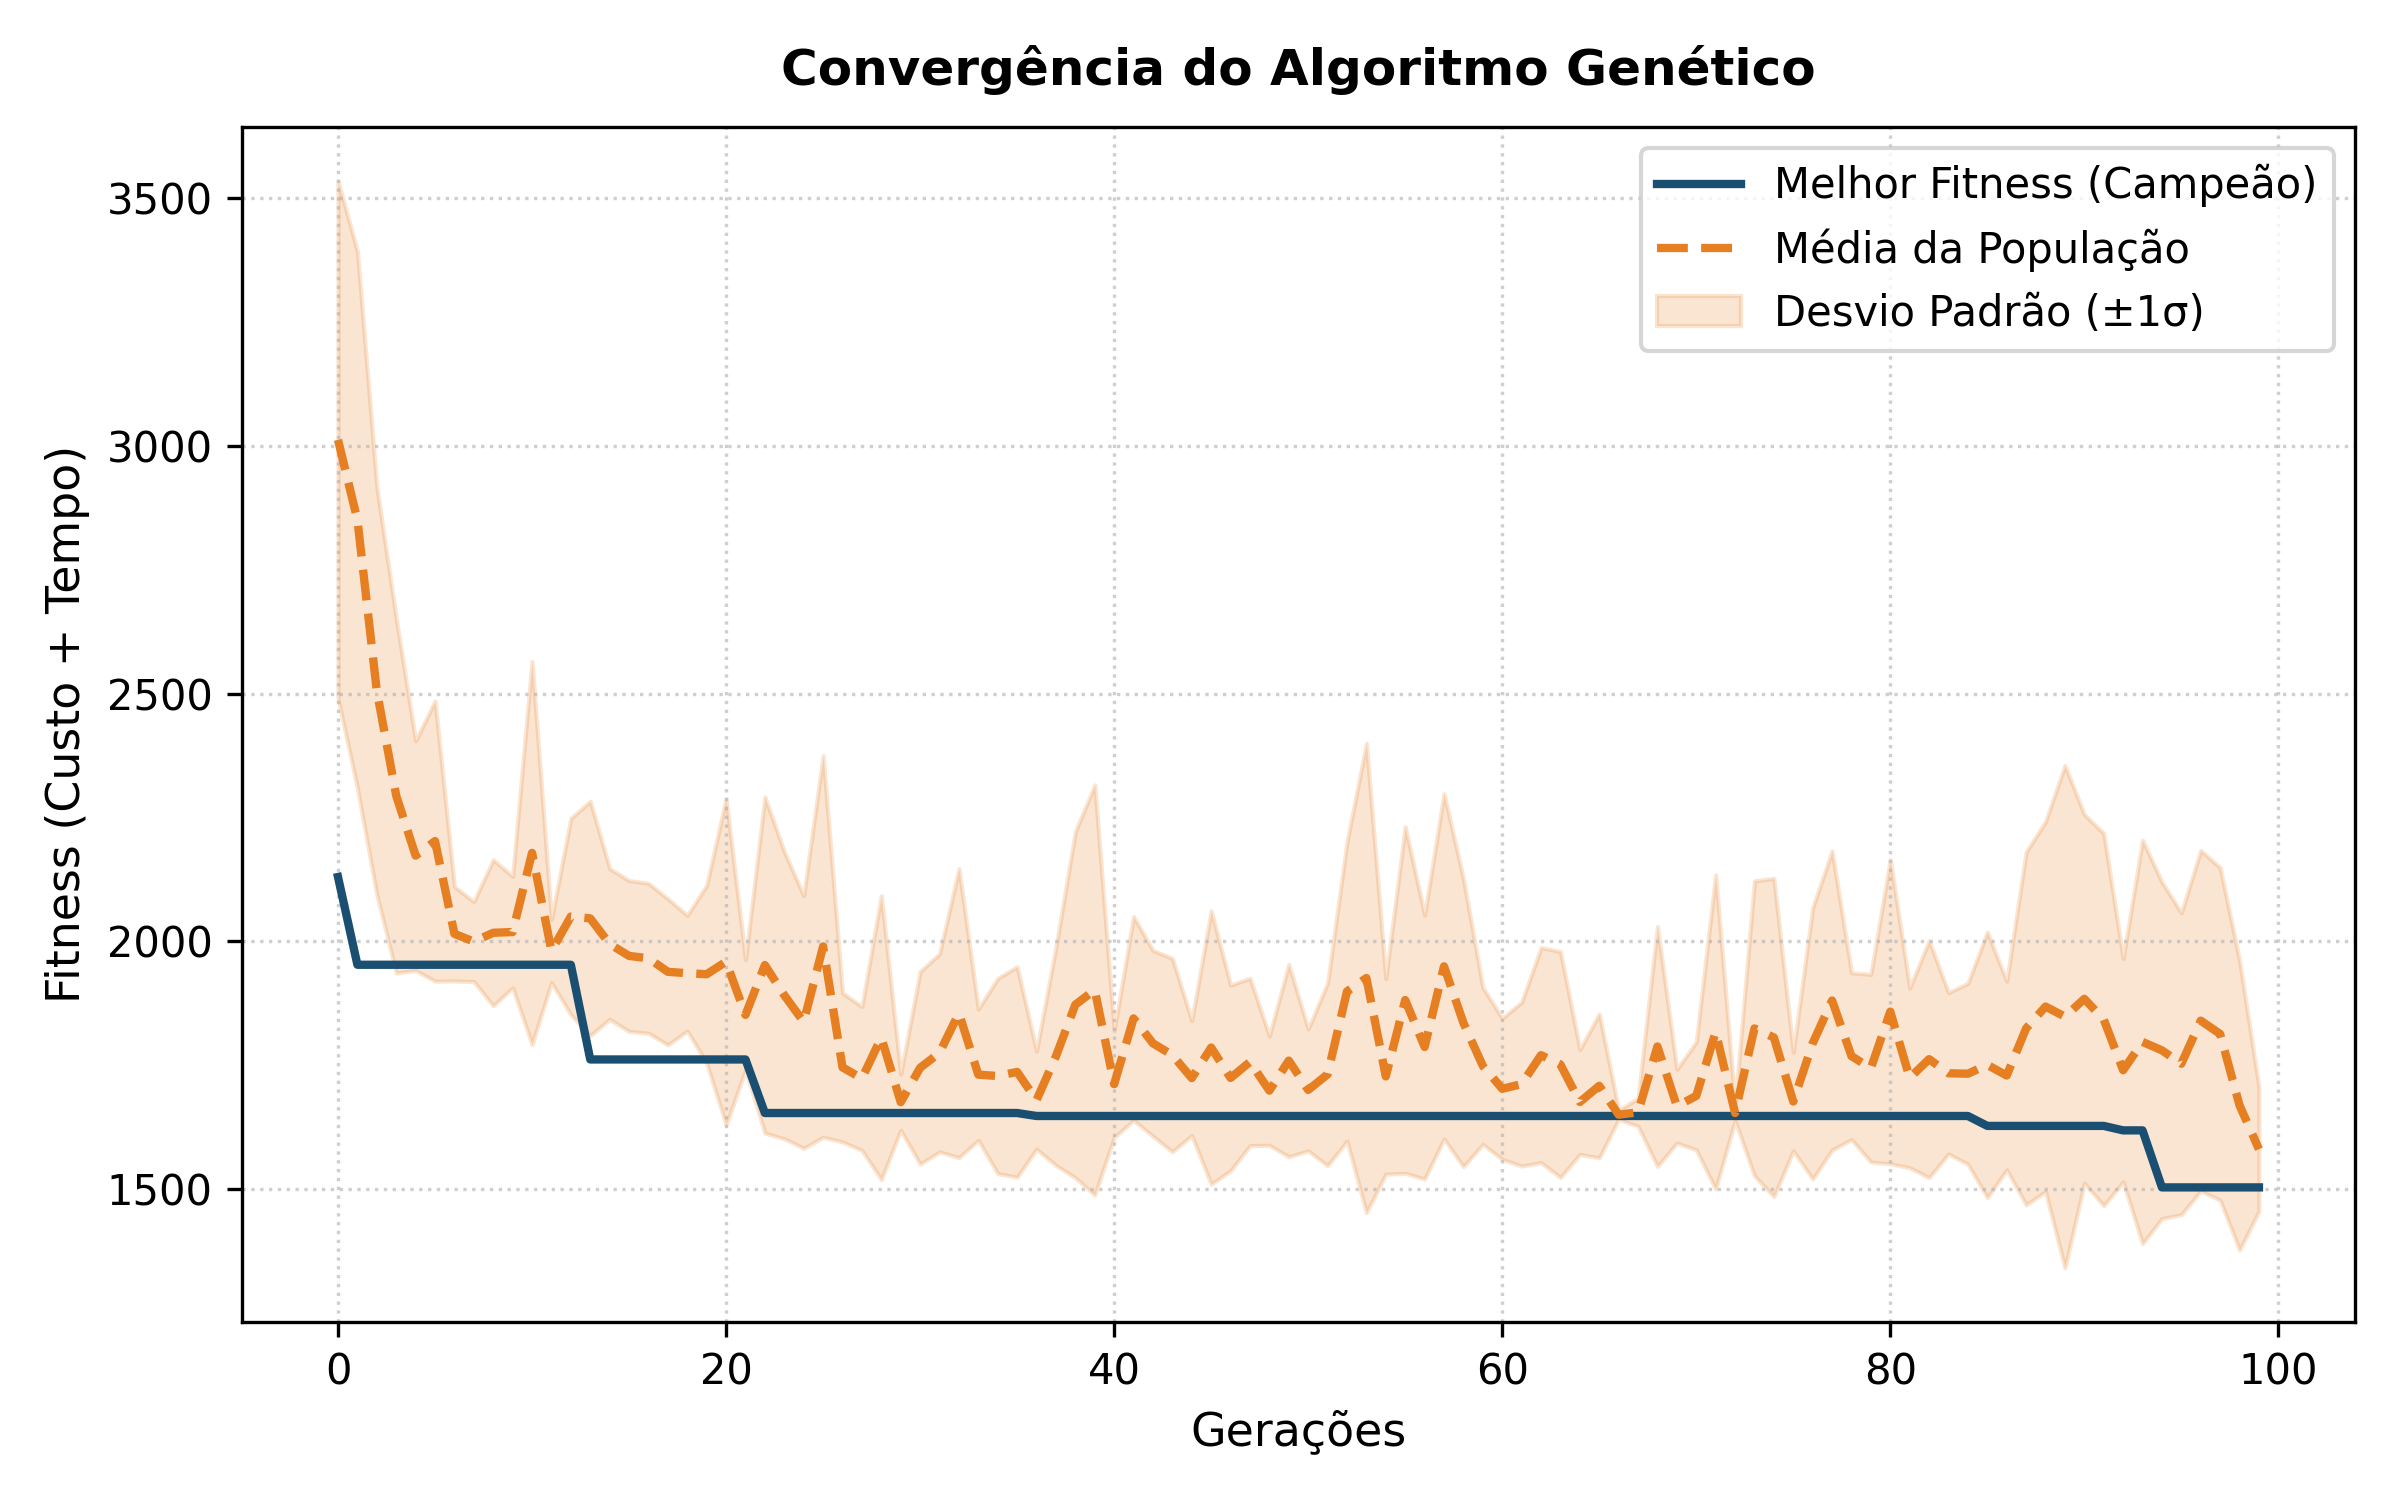
\includegraphics[width=\linewidth]{Imagens/Grafico_1_Convergencia.png}
	
	{\footnotesize Fonte: Autoria Própria (2026).}
\end{figure}


No gráfico da figura 3 é demonstrado a variação genética, através da mutação inserida no algoritmo. 

\begin{figure}[H]
	\centering
	
	\caption{Variância Gerada}
	\vspace{0.2cm}
	
	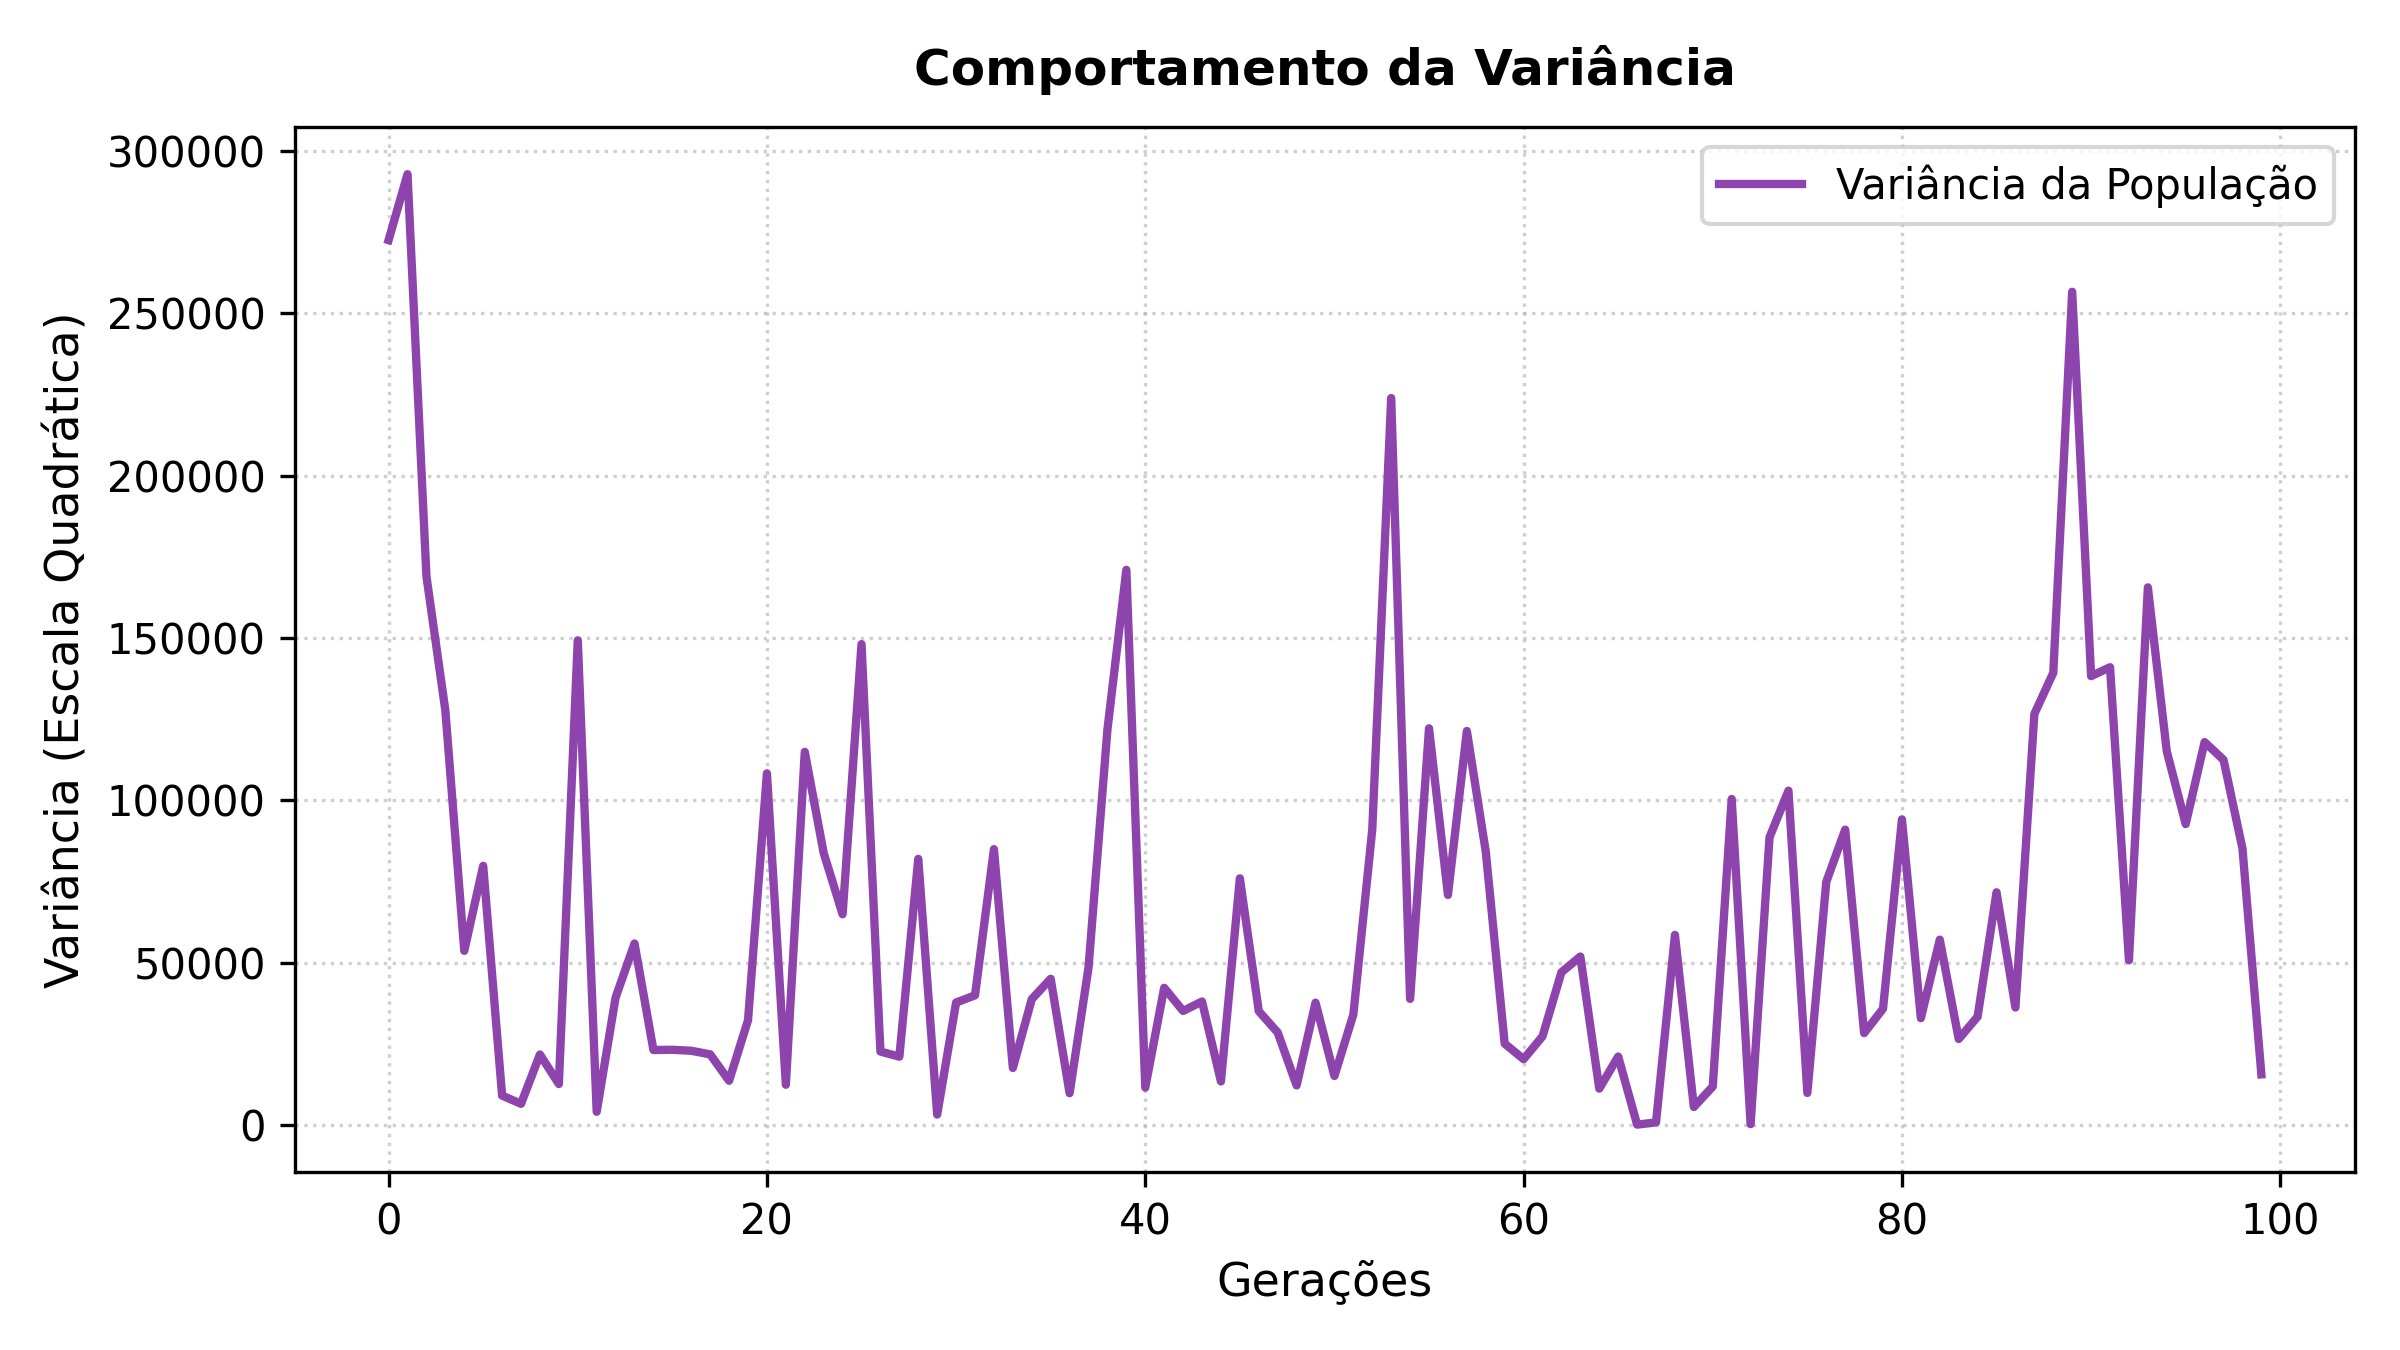
\includegraphics[width=\linewidth]{Imagens/Grafico_2_Variancia.png}
	
	{\footnotesize Fonte: Autoria Própria (2026).}
\end{figure}



%----------------------------------------------------

\section{Conclusão}

Durante o trabalho foi possível verificar o funcionamento do algorítimo genético mudando suas variáveis para observar o seu peso e como deveria ser ajustados conforme o problema.

Foi possível verificar que esse tipo de implementação pode ser usada em diferentes tipos de problemas e com adequações pode ser muito útil, mas deve ser usada com muito estudo de caso pois pode facilmente viram um algoritmo de aleatoriedade sem eficiência.

Foi utilizado um código em python para demonstração visual dos resultados e melhor compreensão das estatísticas com o passar das gerações.  



\begin{thebibliography}{9}
	
	\bibitem{cppreference}
	Cppreference Contributors. \textbf{C++ Reference}. 2026. Disponível em: \url{https://en.cppreference.com/}. Acesso em: 12 jun. 2026.
	
	\bibitem{cplusplus}
	cplusplus.com. \textbf{Reference - C++ Information}. 2026. Disponível em: \url{https://cplusplus.com/}. Acesso em: 12 jun. 2026.
	
	\bibitem{pandas}
	The pandas development team. \textbf{pandas - Python Data Analysis Library}. 2026. Disponível em: \url{https://pandas.pydata.org/}. Acesso em: 12 jun. 2026.
	
	\bibitem{matplotlib}
	Matplotlib Development Team. \textbf{Matplotlib: Visualization with Python}. 2026. Disponível em: \url{https://matplotlib.org/}. Acesso em: 12 jun. 2026.
	
	\bibitem{atividade}
	Disciplina de Inteligência Artificial (ECOI22). \textbf{Atividade Algoritmos Evolucionários}. Material de avaliação disponibilizado via SIGAA. 2026. Atividade baseada no trabalho dos professores Jones Granatyr e Guilherme Matos Passrini.
	
\end{thebibliography}

\end{document}